\section{Introduction}

In the world of short-range communication, a variety of technologies and protocols exist, each designed to serve specific needs. 
While these solutions work well for small-scale applications and localized coverage, they often struggle with interoperability.

Communication technologies today are highly fragmented, with different standards and protocols optimized for different use cases. 
While some technologies provide effective coverage for small areas, seamless integration across networks remains a challenge. 
This has led to the need for a new, unified communication stack that can bridge these gaps.
\begin{figure}[H]
    \centering
    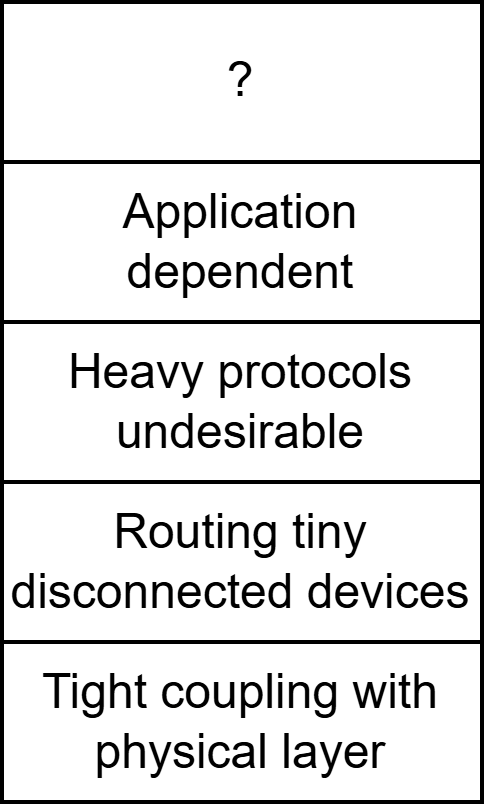
\includegraphics[width=0.25\linewidth]{images/iot13.png}
    \caption{New communication stack}
\end{figure}
\noindent Several communication solutions are available, and they can generally be categorized based on:
\begin{itemize}
    \item Proprietary (WirelessHART) or open standards (WiFi, ZigBee, 6LowPAN, THREAD). 
    \item Application-specific or application-agnostic. 
    \item IP-compliant or not IP-compliant. 
\end{itemize}

\paragraph*{ZigBee and 6LowPAN}
Among the many existing technologies, ZigBee and 6LowPAN are two of the most widely used.
While they share similarities at the lower communication layers, their fundamental difference lies in their approach to IP connectivity:
\begin{itemize}
    \item 6LowPAN extends IP to IoT devices, making it easier to integrate with existing internet infrastructure.
    \item ZigBee, on the other hand, operates independently of IP, requiring additional gateways for internet connectivity.
\end{itemize}